\documentclass[10pt]{article}

\usepackage[english]{babel}										
                                                               
\usepackage[utf8]{inputenc}										
\usepackage[T1]{fontenc}										

\usepackage{amsmath,amsfonts,amssymb,amsthm,cancel,siunitx,
calculator,calc,mathtools,empheq,latexsym}

\usepackage{subfig,epsfig,tikz,float}

\usepackage{booktabs,multicol,multirow,tabularx,array}

\usepackage{hyperref}
\usepackage{natbib}

\usepackage{xcolor}
\usepackage{listings}

\definecolor{mGreen}{rgb}{0,0.6,0}
\definecolor{mGray}{rgb}{0.5,0.5,0.5}
\definecolor{mPurple}{rgb}{0.58,0,0.82}
\definecolor{backgroundColour}{rgb}{0.95,0.95,0.92}

\lstdefinestyle{CStyle}{
    backgroundcolor=\color{backgroundColour},   
    commentstyle=\color{mGreen},
    keywordstyle=\color{magenta},
    numberstyle=\tiny\color{mGray},
    stringstyle=\color{mPurple},
    basicstyle=\footnotesize,
    breakatwhitespace=false,         
    breaklines=true,                 
    captionpos=b,                    
    keepspaces=true,                 
    numbers=left,                    
    numbersep=5pt,                  
    showspaces=false,                
    showstringspaces=false,
    showtabs=false,                  
    tabsize=2,
    language=C
}

\sloppy
\setlength{\parindent}{0pt}
\setlength{\parskip}{5pt}
\textwidth 13.5cm
\textheight 19.5cm
\columnsep .5cm

\title{\renewcommand{\baselinestretch}{1.17}\normalsize\bf%
\uppercase{PageRank and HITS: a comparison}
}

\author{
Giacomo Zanatta - 859156
}

\begin{document}

\date{}

\maketitle

\vspace{-0.5cm}

\begin{center}
{\footnotesize 
IRWS Project - Ca' Foscari University, Venice 
}
\end{center}

% -------------------------------------------------------------------
% Abstract
\bigskip
\noindent
{\small
\url{https://github.com/giacomozanatta/pagerank-hits}
}
\iffalse
\medskip
\noindent
{\small{\bf Keywords}{:} 
}
\fi

\baselineskip=\normalbaselineskip
% -------------------------------------------------------------------

\section{Introduction}\label{sec:1}
The project \cite{Zanatta_Page_Rank_HITS_2022}consists of an implementation of {\bf PageRank}\cite{Page98thepagerank} and {\bf HITS}\cite{Kleinberg1999} ranking algorithm and to compute the jaccard distance between two ranking.

The implementation was written in {\bf C language} with extensibility in mind: effort was made in order to write a library prototype that can be easily expanded adding for example other distance functions or different ranking algorithms.

Since we are dealing with large datasets, the underlying adjancency matrices are represented in a {\bf Compressed Row Storage} (from now, CSR) form in addition to the {\bf mmap} support.

This report is subdivided in 3 main chapter.  
In this section we will provide a brief introduction about the implemented algorithms, giving an high level overview.\\
In the next chapter we discuss about the implementation dissecting the library file and we show an example of utilization.\\
On the last chapter we present some results, comparing the generated ranking using the Jaccard similarity.

\subsection{Algorithms}
Here we will explain the main algorithms used for the project.
\subsubsection{PageRank}
\subsubsection{HITS}
\subsubsection{In-Degree}
\subsubsection{Jaccard Similarity}
\section{Implementation}
\subsection{Input data}
A ranking algorithms works with a set of pages. Every page could have a set of outgoing links. An outgoing links represents a link from a page to another one. 

We can model this by using a directed graph: a page is a node of the graph and an directed edge from page x to page y means that page x has an outgoing link to page y.

Network graph is taken from a text file, we assume that a file is structured as a follows:

\begin{enumerate}
    \item {\bf Must starts with an Header}. Header lines begins with the {\bf \texttt{\#}} character. Header contains useful information like the number of nodes and the number of edges of the graph stored in a special line structured like this:
    \begin{verbatim} # Nodes: X Edges: Y \end{verbatim}
    Where X and Y are two integers that represents respectively the number of nodes and the number of edges.
    File must have only one Header section.
    \item {\bf Must contains a number of edges that matches the number specified in the header}. After the section header, file must contains Y lines (where Y is the number of edges). An edge of the graph is defined by a line in the file. A line after the header must be in the next format:
    \begin{verbatim}A B\end{verbatim}
    Where A and B are two integers. A line in the file says that page identified by ID A has an outgoing link to the page identified by id B. 
    For better understandability, we call A FROMNODEID and B TONODEID
    \item {\bf Edges entry must be ordered}. The entry of the file must be sorted first by the first integer of the line and then by the second one.
\end{enumerate}
Here we provide a simple example of a valid file.
\begin{verbatim}
# Test graph
# Nodes: 8 Edges: 14
# FromNodeId	ToNodeId
0 3
1 2
1 4
2 0
3 1
4 1
4 2
4 3
4 5
5 2
5 7
6 0
6 2
7 0
\end{verbatim}
\subsection{Matrix representation}
The previous example corresponds to the next adajcency matrix:

$ \begin{bmatrix}
    0 & 0 & 0 & 1 & 0 & 0 & 0 & 0 \\
    0 & 0 & 1 & 0 & 1 & 0 & 0 & 0 \\
    1 & 0 & 0 & 0 & 0 & 0 & 0 & 0 \\
    0 & 1 & 0 & 0 & 0 & 0 & 0 & 0 \\
    0 & 1 & 1 & 1 & 0 & 1 & 0 & 0 \\
    0 & 0 & 1 & 0 & 0 & 0 & 0 & 1 \\
    1 & 0 & 1 & 0 & 0 & 0 & 0 & 0 \\
    1 & 0 & 0 & 0 & 0 & 0 & 0 & 0 
    \end{bmatrix}  $

Storing this matrix in a standard matrix representation requires $8*8 = 64$ entries.

Problem arises when we have to work with huge dataset: some network has {\bf millions of nodes} and this requires a lot of space.

For example, if we store entries as a float (4 bytes) a network with 50.000 nodes has 2.500.000.000 entries and we need 4*2.500.000.000 bytes (10 gigabytes) for store them.

Since large matrix are very sparse (we assume that a page contains only a few outgoing links) we can store the matrix in a CSR format.
\subsubsection{CSR format}
Matrices in CSR format are expressed by three one-dimensional array \cite{DongarraSparseMatrix}: one array (val) contains the non-zero values of the matrix. Another array (col\_index) is used to store the column indexes of the elements in the val vector. The last vector (row\_ptr) stores the locations in the val vector that start a row. In a more specific say:
\begin{enumerate}
    \item The arrays val and col\_index are of length N (number of total non-zero values in matrix), and contain the non-zero values and the column indices of those values respectively.
    \item The row\_pointer array is of length (m + 1) (m is the number of row of the matrix) and is defined recursively as:
    \begin{itemize}
        \item $\text{row\_pointer}[0] = 0$
        \item $\text{row\_pointer}[i] = \text{row\_pointer}[i-1] + $number of non-zero elements in the (i-1) th row of the matrix.
    \end{itemize}
\end{enumerate}
For example, the previous defined matrix is represented in CSR format as:
\begin{itemize}
    \item $\text{val}=[1.0,1.0,1.0,1.0,1.0,1.0,1.0,1.0,1.0,1.0,1.0,1.0,1.0,1.0]$
    \item $\text{col\_index}=[3,2,4,0,1,1,2,3,5,2,7,0,2,0]$
    \item $\text{row\_pointer}=[0,1,3,4,5,9,11,13,14]$
\end{itemize} 
On the next subsection we analize how the CSR is created from the dataset and we give an overview of the library.
\subsection{Library Structure}
The library provides some header files that contains some function and data structures used for ranking computation.
The header files are:
\begin{enumerate}
    \item {\bf dataset.h}: provides function for parsing the file and to generate a Dataset struct.
    \item {\bf csr.h}: provides function to generate a csr struct from a dataset and the stochastization method used for page rank.
    \item {\bf ranking.h}: provides ranking functions and similarity computations between ranking.
    \item {\bf utils.h}: provides utils stand-alone functions.
    \item {\bf constants.h}: in this header some constants are defined.
\end{enumerate}
The header files and implementations are discussed in the next subsection.
\subsubsection{Dataset}
The dataset struct contains this attributes:
\begin{enumerate}
    \item int** DATA: this represents the set of entries of the dataset. An entry is a single line of the file and consists of an array with length 2: the first one is the FROMNODEID, the second one is the TONODEID. This is not always the case: if we read the transpose dataset, the two elements of the array are swapped.
    \item int n\_nodes: number of nodes in the dataset.
    \item int n\_edges: number of edges in the dataset.
    \item char* name: the name of the dataset. It is generated from the file name.
\end{enumerate}
The Dataset header provides the next functions:
\begin{enumerate}
    \item int read\_dataset\_from\_file(char *file\_path, DATASET* dataset, int order): reads the dataset from the given file. Order parameter can be used to obtain a transposed dataset: order can be 0 (standard order), or 1 (transposed order). User can use the defined costants for the order: TO\_NODE\_ID\_FIRST and FROM\_NODE\_ID\_FIRST. This function will populate the n\_nodes and n\_edges from the header of the file and it will copy the dataset entries inside the DATA array, allocating memory. 
    \item void sort\_dataset(DATASET *dataset): this function will sort the dataset using quicksort.
    \item void destroy\_dataset(DATASET* dataset): it will free the memory used by the dataset.
    \item void print\_dataset(DATASET dataset): debug function that print out the dataset in standard output.
\end{enumerate}
\subsubsection{Csr}
The CSR struct contains this attributes:
\begin{enumerate}
    \item float* val: the val array, of size n\_cols.
    \item int *col\_index: the col\_index array, of size n\_cols.
    \item int *row\_ptr: the row\_ptr array, of size n\_rows + 1.
    \item int n\_rows: number of rows in the matrix.
    \item int n\_cols: number of columns in the matrix.
\end{enumerate}
The CSR header provides the next functions:
\begin{enumerate}
    \item int csr\_from\_dataset(DATASET dataset, CSR* csr): creates a CSR from a dataset, allocating the memory for the arrays.
    \item int make\_stochastic(CSR* csr): make the CSR matrix stochastic. This is used for PageRank computation. It will transforms every values in the val array with 1/(number of elements in the row of the entry). For example, the value array defined in section 2 (CSR format) after calling the make\_stochastic function it will be transformed into:
    
    $\text{val}=[1.0,1/2,1/2,1.0,1.0,1/4,1/4,1/4,1/4,1/2,1/2,1/2,1/2,1.0]$
    Note that the sum of the entries of every row is equal to 1.
    \item int destroy\_csr(CSR* csr): frees the memory used by the CSR matrix.
\end{enumerate}
\paragraph{About mmap}
The mmap feature is implemented using compile vars. It was done this way for not change too much the implementation and to permits a standard usage of the library, without having functions redecleration that will make the library utilization more complex.
For enabling the mmap on CSR data structured, user must compile the source with the -DMMAP flag.
Please note that mmap will creates the next files inside the folder of the dataset file:
    \begin{enumerate}
        \item \{fileName\}Scol: for the col\_index array.
        \item \{fileName\}Srow: for the row\_pointer array.
        \item \{fileName\}Sval: for the val array.
        \item \{fileName\}Tcol: for the col\_index array of a transposed csr.
        \item \{fileName\}Trow: for the row\_pointer array of a transposed csr.
        \item \{fileName\}Tval: for the val array of a transposed csr.
    \end{enumerate}
where \{fileName\} is the name of the file.
\subsubsection{Ranking}
The Ranking type is defined as an array of RankEntry.
A RankEntry is defined as a struct with two attributes:
\begin{enumerate}
    \item int ID: the ID of the page
    \item float value: the ranking of the page
\end{enumerate}
The ranking header provides the next functions:
\begin{enumerate}
    \item int pagerank(CSR csr, Ranking* P, int* n\_iter): computes the PageRank from the given CSR. It will store the ranking in the P variable, and the number of iterations to converge is returned inside the n\_iter variable.
    \item int hits(CSR csr, CSR csr\_transpose, Ranking* A, Ranking* H, int *n\_iter): computes the HITS hub and authority ranking. These ranking are returned in the A and H variable respectively. It needs the CSR and the transposed CSR.
    \item int indegree(CSR csr, Ranking* I): computes the Indegree (returned inside I) of the given CSR.
    \item void sort\_ranking(Ranking R, int n): it will sorts the RankEntries of the Ranking variable by value, decreasing order.
    \item double jaccard\_score(Ranking A, Ranking B, int k): it will compute the Jaccard Score of two ranking limited to position K.
\end{enumerate}
\subsubsection{Constants and Utils}
The constants and utils header provides some defined constants intended to use for communicating with the library and some common functions used by the library.
\section{Utilisation of the library}
The library is shipped out with a simple main that shows how the library is intended to use.

Firstly, an user needs to load the dataset. He must create a variable of type Dataset and pass the pointer of it to the function read\_dataset\_from\_file specifying also the file name and the order: TO\_NODE\_ID\_FIRST order is the standard one. FROM\_NODE\_ID\_FIRST is used for load the dataset transpose.

After initializing the dataset struct, he can create the CSR matrix by calling the csr\_from\_dataset function passing the dataset and a pointer to a CSR struct, for example the next lines of code:
\begin{center}
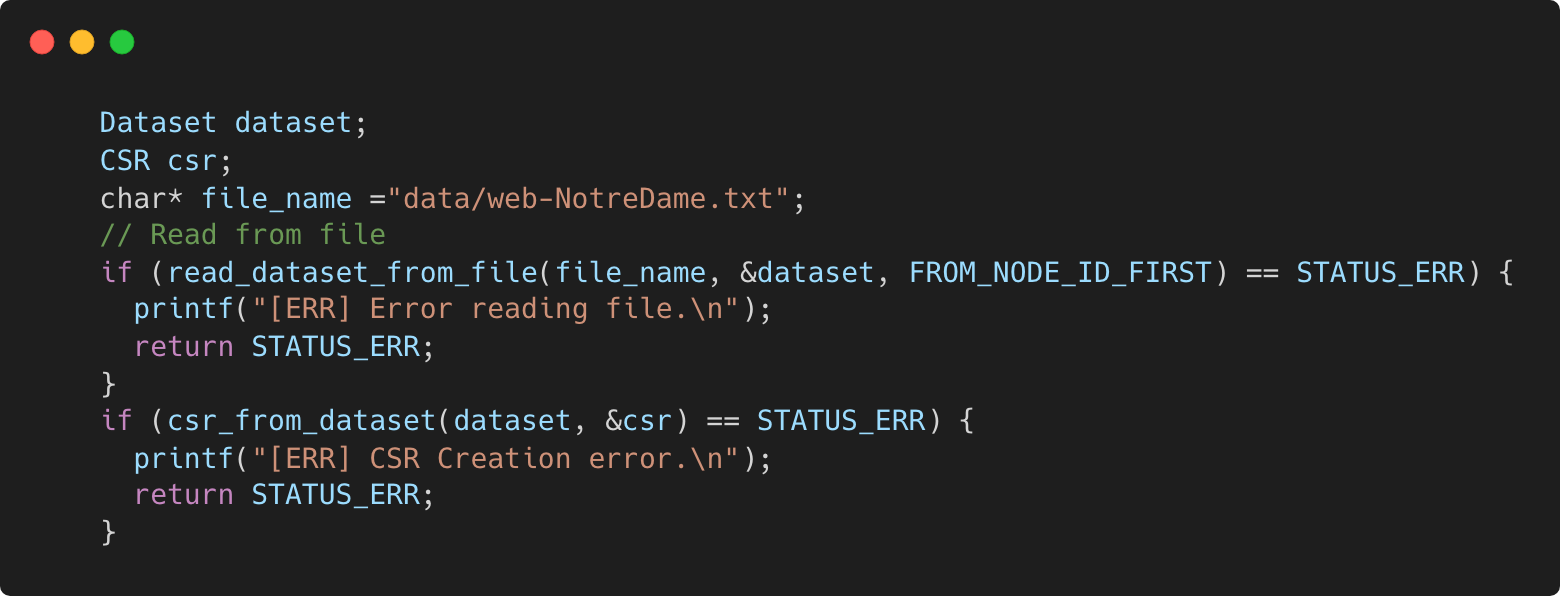
\includegraphics[scale=0.2]{img/main-1-ex.png}
\end{center}
will load the dataset from file data/web-NotreDame.txt into the dataset variable and it will create the CSR struct from the given dataset.

After that, user can use the CSR for compute a rank. For example, if user wants to compute PageRank he can firstly make the CSR stochastic with the appropriate function and then call the page\_rank function.
\begin{center}
    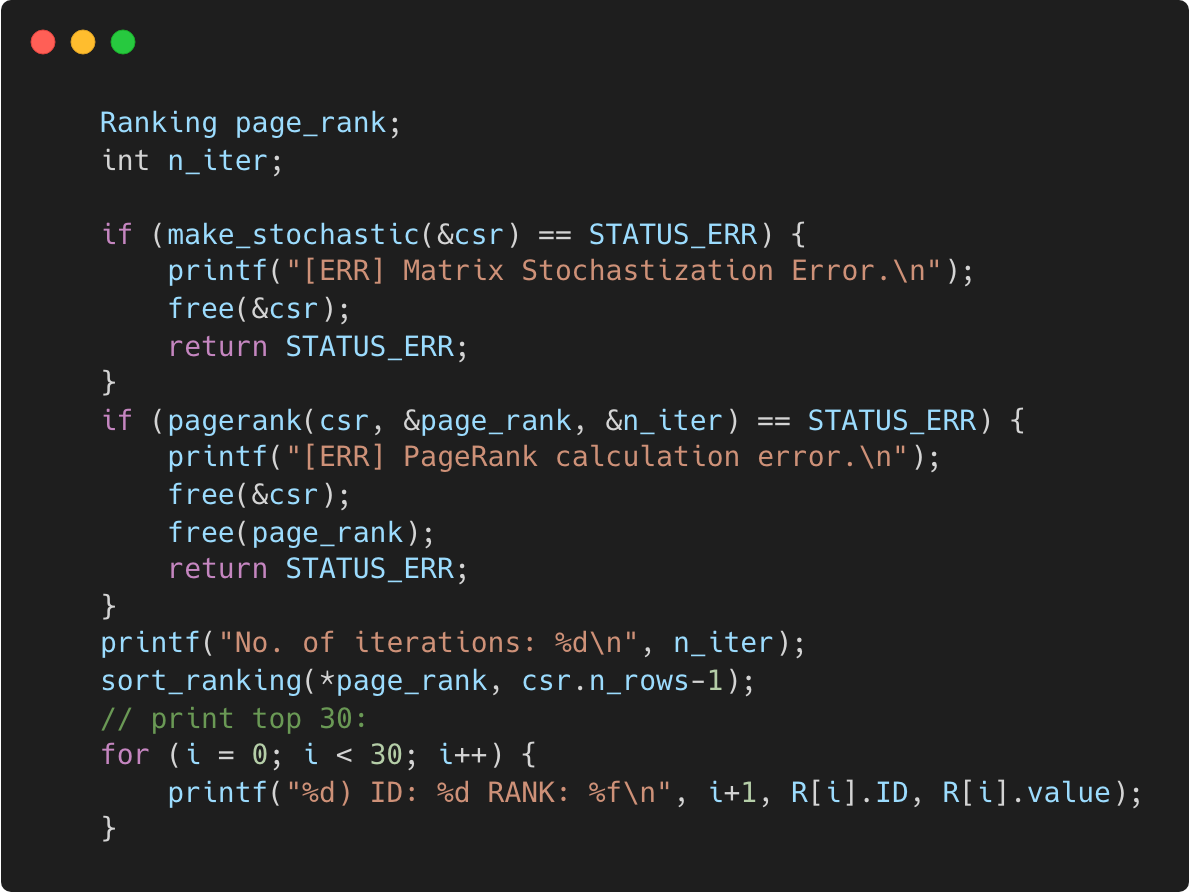
\includegraphics[scale=0.2]{img/main-2-ex.png}
\end{center}
The previous image shows how to use to print out the top k pages: user must sort the ranking and then iterate over the Ranking array.
The Jaccard Similarity between two Ranking can be computed by calling:  
\begin{center}
    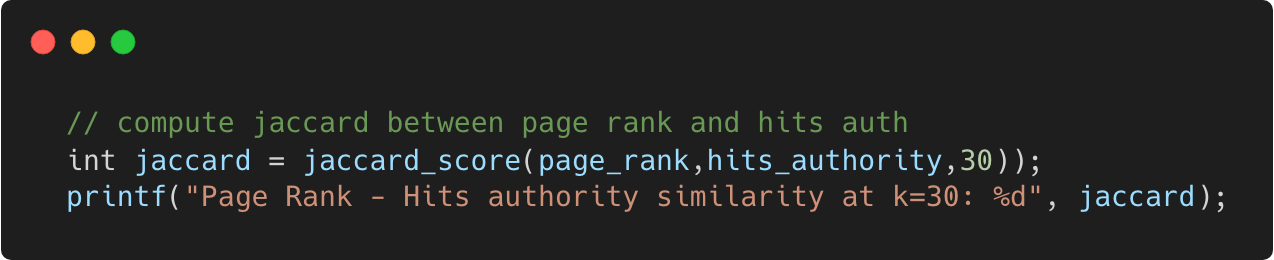
\includegraphics[scale=0.2]{img/main-3-ex.png}
\end{center}

\subsection{The main file}

\subsection{Building the demo}
The demo program can be builded by launching the make command from the command line.
User can open a new terminal window from the project directory and launch the next command:
\begin{verbatim}make\end{verbatim}
for building the project. This command reads the MakeFile and executes the default rule.

For using the mmap feature, user must call from the terminal
\begin{verbatim}make mmap\end{verbatim}
The two commands mentioned before generates, respectively, two executable files:
\begin{enumerate}
    \item {\bf ranking:} the demo program with standard feature.
    \item {\bf ranking-mmap:} the demo program with mmap feature.
\end{enumerate}

\subsection{Executing the demo}
User must launch the program passing two parameters as arguments: the first one is the path of the input file and the second one is an integer K used for print out the K-top ranking and to compute similarity, for example:
\begin{verbatim}./ranking data/web-NotreDame.txt 30\end{verbatim}
it will launch the default version of program (without mmap) using the dataset data/web-NotreDame.txt and with the top 30 ranking printed out.
\section{Some results}
Now we analyze the dataset web-NotreDame. 

The top 30 pages returned by page rank are:

The top 30 pages returned by HITS are:

The top 30 pages returned by InDegree are:

The Jaccard similarity values returned are:
\begin{enumerate}
    \item PageRank - HITS authority
        \begin{enumerate}
            \item K=10:
            \item K=20:
            \item K=30:
        \end{enumerate}
    \item HITS authority - InDegree
        \begin{enumerate}
            \item K=10:
            \item K=20:
            \item K=30:
        \end{enumerate}
    \item PageRank - InDegree
        \begin{enumerate}
            \item K=10:
            \item K=20:
            \item K=30:
        \end{enumerate}
\end{enumerate}
\section{Conclusion}
\newpage

% -----------------------------
\bibliographystyle{abbrv} 
\bibliography{references.bib} % Bibliography

\end{document}